\documentclass[12pt, a4paper, hidelinks]{article}

% Packages:
\usepackage{graphicx}                   % For figure includes
\usepackage[T1]{fontenc}                % For mixing up \textsc{} with \textbf{}
\usepackage[utf8]{inputenc}             % For scandinavian input characters(æøå)
\usepackage{amsfonts, amsmath, amssymb} % For common mathsymbols and fonts
\usepackage[danish]{babel}              % For danish titles
\usepackage{hyperref}                   % For making links and refrences
\usepackage{url}                        % Just because {~_^}
\usepackage{array}                      % ...
\usepackage[usenames, dvipsnames, svgnames, table]{xcolor}
\usepackage{tabularx, colortbl}
\usepackage{verbatim} % For entering code snippets.
\usepackage{fancyvrb} % A "fancy" verbatim (for pseudo code).
\usepackage{listings} % For boxed codesnippets, and file includes. (begin)
\usepackage{lipsum}   % For generating dummy text at this demonstration
\usepackage{scrextend} % For den fede liste type
\usepackage{placeins}



% Basic layout:
\setlength{\textwidth}{165mm}
\setlength{\textheight}{240mm}
\setlength{\parindent}{0mm}
\setlength{\parskip}{\parsep}
\setlength{\headheight}{0mm}
\setlength{\headsep}{0mm}
\setlength{\hoffset}{-2.5mm}
\setlength{\voffset}{0mm}
\setlength{\footskip}{15mm}
\setlength{\oddsidemargin}{0mm}
\setlength{\topmargin}{0mm}
\setlength{\evensidemargin}{0mm}

\newcolumntype{C}[1]{>{\centering\arraybackslash}p{#1}}

% Colors:
\definecolor{KU-red}{RGB}{144, 26, 30}

% Text Coloring:
\newcommand{\green}[1]{\textbf{\color{green}{#1}}}
\newcommand{\blue} [1]{\textbf{\color{blue} {#1}}}
\newcommand{\red}  [1]{\textbf{\color{red}  {#1}}}

% Simple Language Highlighting for F#
\definecolor{bluekeywords}{rgb}{0.13,0.13,1}
\definecolor{greencomments}{rgb}{0,0.5,0}
\definecolor{turqusnumbers}{rgb}{0.17,0.57,0.69}
\definecolor{redstrings}{rgb}{0.5,0,0}
\lstdefinelanguage{FSharp}
                  {morekeywords={let, new, match, with, rec, open,
                      module, namespace, type, of, member, and, for,
                      in, do, begin, end, fun, function, try, mutable,
                      if, then, else},
                    keywordstyle=\color{bluekeywords},
                    sensitive=false,
                    morecomment=[l][\color{greencomments}]{///},
                    morecomment=[l][\color{greencomments}]{//},
                    morecomment=[s][\color{greencomments}]{{(*}{*)}},
                    morestring=[b]",     stringstyle=\color{redstrings}
                  }
% You might want to change these lines at some point
\lstset{
  basicstyle=\ttfamily,
  columns=fullflexible,
  keepspaces=true,
  language=FSharp
}

% ************************* Start Document *****************
\begin{document}

% ************************* Page Header ********************
\begin{minipage}[b]{1.0\linewidth}

\includegraphics[height=30mm]{KULogo}

\vspace*{-16ex}
\begin{center}
    {\Large \bf Programmering og Problemløsning} \vspace*{1ex} \\
    {\large Ugeopgave 1} \vspace*{1ex} \\
    {\large Frederik Kallestrup Mastratisi, Aiyu Liu og Rasmus Frydendal Kristensen}
\end{center}
\vspace*{-3pt}
{\color{KU-red}\hrule}
\end{minipage}
\vspace{2ex}

% **************** Assignment Starts Here ******************
\tableofcontents \newpage

\setcounter{section}{1}
\setcounter{subsection}{-1}



\subsection{Links til koden}

1.1: \url{https://scratch.mit.edu/projects/121224396/#editor} \\

1.2: \url{https://scratch.mit.edu/projects/120071859/#editor} 

\vspace{10mm}





\subsection{Hvad kan I lave med 10 blokke?}

I Figur 1 ser I 10 Scratch blokke. Jeres opgave er at lave et sjovt program, kun ved
brug af disse blokke. Hver blok må bruges 0, 1 eller flere gange. Prøv at sammensætte
programmet ved at tegne blokkene på papir, og skriv ned, hvad I tror programmet
vil gøre. Sæt jer dernæst til computeren, og indtast jeres program. Beskriv, i hvor
høj grad programmet gør, som I forventede. Vend dernæst tilbage til designfasen og
forbedre evt. programmet. Til slut uploades programmet til gruppens rum i Scratch

\vspace{10mm}

Vi ville have lavet to "when-this-sprite-clicked" blokke, således at den en ene clicked blok kontrollerede kattens bevægelse og den anden clicked-blok stod for at katten kunne lave sin meow lyd, mens den bevægede sig. Men ved nærmere eftertanke, fandt vi ud af at katten bare ville sige meow og derefter starte dens bevægelser på ny - idet et click på katten ville aktivere begge "when-this-sprite-clicked" blokke.  
I stedet besluttede vi os for at arbejde med én "when-this-sprite-clicked" blok.

På forhånd havde vi designet koden på et stykke papir, ved implementering i Scratch ser det ud således:

\begin{figure}
  \begin{center}
    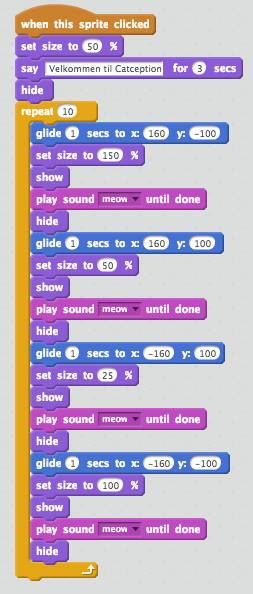
\includegraphics[width=70mm]{B1.png}
  \end{center}
  \caption{}
  \label{fig:B1}
\end{figure}

\FloatBarrier
Programmet skulle forløbe således at kattens størrelse fra start blev sat til 50 procent og sige "Velkommen til katception". Derefter skulle katten skjule sig og glide hen til det første hjørne - nederst til venstre, vise sig igen i en anden størrelsesformat og sige meow. Sådan skulle det gerne fortsætte i alle fire hjørner, således at katten bevæger sig fra det sydøstllige til det nordøstlige til det nordvestige til det sydvestlige hjørne. Effekten af dette skulle gerne være at katten pludseligt popper up på skærmen og siger meow i en anden størrelsesformat hver gang. Med repeat sat til 10, er det intentionen at katten skal bevæge sig 10 gange rundt omkring de 4 hjørner.

Det kører perfekt, akkurat som forventet! Programmet i sig selv er meget simpelt og kræver ingen kompleks matematik. Det indeholder også kun én sprite, så overvejelser omkring hvilken kode der skal implementeres til hvilken sprite er der også fritaget for.

For at gøre programmet ekstra sjovt implementeres "Leo" "nardo" "di" "Catprio!!!" hvert for sig ved hvert hjørne før meow lyden:

\begin{figure}
  \begin{center}
    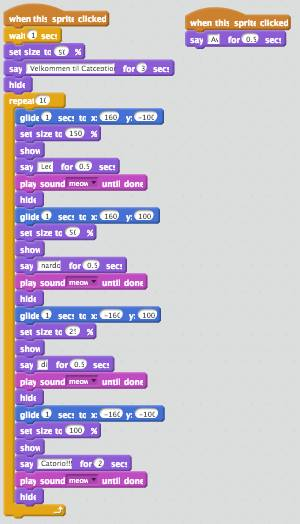
\includegraphics[width=70mm]{B2.png}
  \end{center}
  \caption{}
  \label{fig:B2}
\end{figure}

\FloatBarrier

Vores oprindelige idé med to "when-this-sprite-clicked" blokke blev ikke realiseret. Til sidst besluttede vi os for at gøre det alligevel med en "when-this-sprite-clicked" blok der skulle stå for at katten nu kunne sige "Av" og samtidigt genstarte det første "when-this-sprite-clicked" blok. Men det voldte en smule problemer, idet katten ikke ville sige "Velkommen til Catception" ved genstart. Vi tænkte det havde noget med samtidigheden af deres køretider ved click at gøre. Ved at lade det første "when-this-sprite-clicked" blok vente i et sekund blev det dermed fixet. 

Den endelige kode:

\begin{figure}
  \begin{center}
    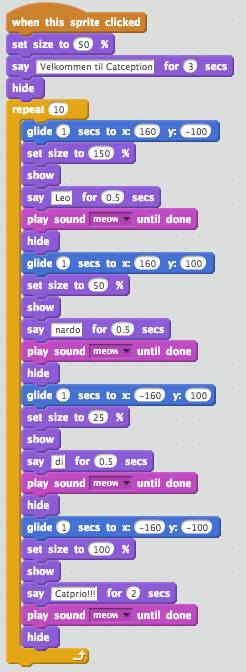
\includegraphics[width=70mm]{B3.png}
  \end{center}
  \caption{}
  \label{fig:B3}
\end{figure}

\FloatBarrier

\subsection{Design et spil}

I skal designe og implementere et spil efter eget valg. Spillet skal indeholde 2-5
sprites, vare ca. 1 minut at spille og må benytte alle tilgængelige blokke i Scratch.
Det må gerne minde om et spil I kender, og det er ikke vigtigt at det er et grafisk
eller lydmæssigt prangende spil. Start med at tale om hvad I kunne tænke jer,
spillet skal omhandle. Skitser på papir, hvordan game-playet, skal forløbe. Skitser
derefter på papir hvordan det kunne implementeres i Scratch. Indtast programmet
på computeren og afprøv, om spillet gør, som I forventer. Vend tilbage til designfasen
og forbedre evt. spillet.

\vspace{10mm}

Spil bsekrivelse

Vi har lavet et simpelt spil, hvor en kat skal hoppe på tilfældigt genererede klaverer for at undvige zombier.


\vspace{10mm}

Inden vi begyndte at kode spillet, lavet vi en skitsering hvor vi skrev de features vi gerne ville have med i spillet. 
\vspace{5mm}
\\ De er som nedenstående:
\begin{labeling}{Skifte image / animation  }
\item	[Hoppe]  					Katten kan hoppe og ændre 'animation-state'
\item[Interagere med Blokke] 		Hoppe oven på dem og ned igen
\item[Skifte image / animation]		Oscillerer mellem forskellige 'animation-states', så det visuelt ligner at katten bevæger sig 
\item[Monstre] 					Interagere med monstre - hvis ikke de hoppes over så mister man liv
\item[Pointsystem]  				Efter hvem der har overlevet længst tid
\item[Sværhedsgrad]  			Flere mobs efter tid
\item[Spillets slut]  				Når man har mistet alle sine liv
\end{labeling}

\vspace{10mm}

Dette var de ting vi startede med at ville implenterer, men under kode processen blev disse features  droppet:
\begin{labeling}{Skifte image / animation  }
\item[Pointsystem]  				Når man belønner spillere kan man enten vælge at gøre det med gulderoden eller pisken. Når man har et pointsystem bruger man gulderoden. Vi fandt det lettere at implementere en pisk, i form af at mobs'ene råber af spilleren at han er dårlig når han mister liv
\item[Sværhedsgrad]  			Vores spawn system er lavet således at dette let kunne implementeres, vi valgte dog at lade være, da vi fandt spillet sjovest på den sværeste sværhedsgrad hele tiden
\end{labeling}


\subsubsection{Problemer vi stødte på under kodningen}

\begin{enumerate}

\item Vi forsøgte at implementere hit detection i mob spriten, men dette ville ikke virke, sandsynligvis grundet måden kloner virker i scratch; hit detection virkede kun på den originale mob sprite som vi brugte til at spawne mobsene som katten skulle hoppe over. I stedet forsøgte vi at eksekvere samme funktionalitet fra vores katte sprite  - ved hjælp af messages som blev fanget af den originale mob sprite - hvilket virkede fint. 


\item Vi forsøgte at implementere en point system, ved at den orginale mob sprite - som vi har sat i hjørnet af skærmen-  hele tiden printede ens scorer på skærmen i form af en talebobel. Dette virkede ikke som vi forventede, da alle dens childrens også sagde beskeden. Vi fandt dog en løsning i form af "pisken": Netop at alle mobs gav en negativ besked til spilleren når hit detection blev udløst.


\item Nu hvor mobs'ene gav en besked til spilleren, ville vi gerne have at de ikke alle sammen gav den samme besked. Vi lavde et forsøg hvor vi genbrugte kode fra vores random mob/block spawn system, til at få mobsene til tilfældigt at vælge i mellem nogle beskeder vi havde givet dem på forhånd. Vi ville se om vi kunne for de forskellige childs af den originale mob, og den originale mob selv, til at sige forskellige beskeder når hit detectionen blev udløst, eller om de alle var tvunget til at vælge den samme besked. Fosøget lykkes og de kunne sige forskellige beskeder. Vi valgte derfor at bruge koden til den endelige version af spillet. 


\item Strategien vi valgte til at starte med, med vores animationssytem til katten, var at de forskellige tråde skulle stå for at skifte animations state på katten. Dette virkede ikke optimalt, da concurency problemer introducerede lagg og små bugs til systemet. Vi valgte derfor en ny løsning hvor vi lavede en ny tråd, som var den eneste som stod for at skifte animationsstate på katten. Den måde den vidste om den skulle skifte animationsstate til f.eks. hoppe animationen, var ved at hoppe tråden ændrede i en variable som funktionelt virkede som en bool, og på den måde kunne animationstråden vide hvilket state katten skulle være i.

\item stopklodsen blev som en fejl sat nederst i kode sekvenserne, hvilket gjorde det muligt at køre ``hoppe'' og ''drop ned'' koden en ekstra gang.



\end{enumerate}

\subsection{Beskrivelse af kode}

I Scratch ligger koden i sprites, og hver sprite kan kører flede tråde af kode. I vores spil har vi 3 sprites: \vspace{10mm} \\ Katte-sprite (også kendt som Catman) \\ Piano (blokkene som Catman kan hoppe op på) \\ Mob-spriten (Fjenden i spillet) \vspace{10mm}
\\ I underafsnitene nedenunder vil vi gennemgå de forksellige 'kode-tråde' tilhørende de 3 sprites.

\subsubsection{Katte-spriten (KS)}

KS indeholder i alt 7 forskellige tråde: \vspace{10mm}

\begin{description}
\item[Initialiserings-tråden] Denne tråd er meget simpel, da det eneste den står for er at nulstille variablerne til deres start værdi. Læg mærke til at LivesLeft variablen sættes til 8, selvom Catman har 9 liv. Dette er fordi koden som tjekker hvornår Catman er død ser således ud "LivesLeft < 0" (Se mob-hit-detect tråden).

\begin{figure}
  \begin{center}
    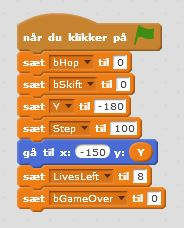
\includegraphics[width=70mm]{TKatInit.jpg}
  \end{center}
  \caption{Initialiseringen af kattens variabler}
  \label{fig:sample}
\end{figure}
 \FloatBarrier

\item[Animations-tråden] Denne tråd står for at bestemme og sætte animations-staten på Catman. Dette gør den ved at gå i gennem en evig løkke som først tjekker om Catman er ved at hoppe. \\

\begin{figure}
  \begin{center}
    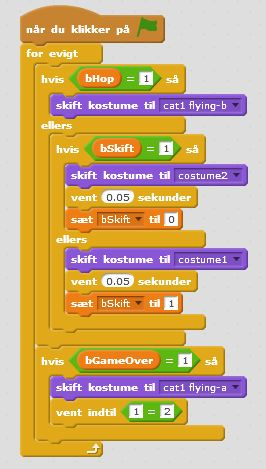
\includegraphics[width=70mm]{TKatAnim.jpg}
  \end{center}
  \caption{Animation af katten}
  \label{fig:TKatAnim}
\end{figure}
\FloatBarrier

 Hvis Catman ikke er ved at hoppe går den ind i et if-else udtryk hvis konditionsudtryk hele tiden skifter mellem at være sand eller falsk hvergang if-else udtrykket eksekveres. If-else udtrykket står for at skifte mellem de 2 animations tilstande som bliver brugt i Catmans løbe animation. \\

 Til sidst i den evige løkke tjekker koden om spillet er i GameOver tilstanden, hvis den er det skifter Catman om til dødsanimations tilstanden, og en linje kode som fungere som en stop klods - og stopper hele tråden- sørger for at Catman ikke skifter animationstilstand derfra, indtil initialiserings-tråden bliver kørt igen (hvilket den vil blive når spillet bliver genstartet).



\item['Hoppe op'-tråden (HO-tråden)]  HO-tråden (eksekverer når spilleren trykker 'pil-op') står for at signalere til resten af trådene at Catman er i gang med at hoppe. Den gør dette ved at sætte bHop (b står for boolean) til 1 i starten af sin eksekvering og derfter til 0 inden den slutter. Inden dette har den dog noget kode som gør at spilleren ikke han hoppe hvis Catman er død, ved at den fryser HO-tråden.\\  

HO-tråden står også for flytte Catman op og ned i hoppet med glide-blokke og for at starte 'piano-blok' kollisionsdetektions-tråden, når Catman er ved et højde punkt 

\begin{figure}
  \begin{center}
    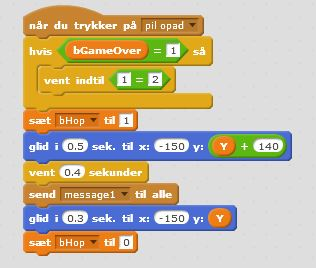
\includegraphics[width=70mm]{TKatPilOp.jpg}
  \end{center}
  \caption{}
  \label{fig:sample}
\end{figure}
\FloatBarrier

\item[ 'piano-blok' kollisionsdetektions-tråden (PbKD-tråden)] PbKD-tråden står for at ændre på Y-variablen i det tilfælde Catman er over en piano-blok, således at han ender med at stå oven på blokken, og bliver udløst af HO-tråden når Catman er ved sit højdepunkt. \\ 

\begin{figure}
  \begin{center}
    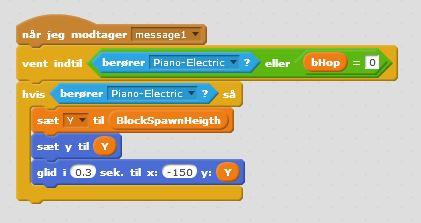
\includegraphics[width=70mm]{TKatPianoColDetect.jpg}
  \end{center}
  \caption{}
  \label{fig:sample}
\end{figure}
\FloatBarrier

Den gør dette ved at vente indtil Catman rør piano-blokken, eller at Catman er færdig med at hoppe (i.e. ikke er i hoppe-tilstand mere). Grunden til at den gør det sidste er således at Catman ikke bare tilportere op til klodsen i det tilfælde at han ikke har ramt nogen klods i sit hop, men rør en imens han er på 'gulvet'. \\ Koden tjekker så om den har fået lov til at gå vidre fordi hoppet er slut, eller fordi den har ramt en klods på vejen ned. Hvis Catman har ramt en klods sætter PbKD-tråden Y-variabel til y-værdien af piano blokkenes spawnhøjde, og sætter Catmans y-koordinat til Y-variablen. Grunden til at der kommer en glide-kommando efter er pga. af concurency problemer, som bliver løst af denne kommando.

\item['Catman står i luften'-tråden (CSL-tråden)] CLS-trådens funktion er at få Catman til at falde ned til gulvet når han står i luften. I.e. når der ikke er nogen piano-klods under catman og når han ikke er igang med at hoppe.  \\

Den måde det virker på er at der en evig lykke som hele tiden venter på at Catman ikke rør en piano-klods og at han ikke er ved at hoppe (altså når bHop = 0). Hvis det er sandt nulstiller CLS-tråden Y-variablen til gulv koordinaterne og sætter en glide-kommando til Y. 

\item['Mob-hit-detektions'-tråden (MHD-tråden)] MHD-tråden funktion er både at holde øje med om Catman er død (når hans antal liv er under 0), og om han har ramt en mob. \\

\begin{figure}
  \begin{center}
    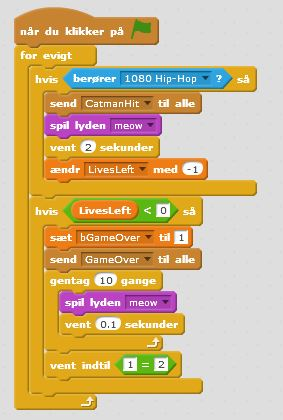
\includegraphics[width=70mm]{TKatMobColDetectOgLiv.jpg}
  \end{center}
  \caption{}
  \label{fig:sample}
\end{figure}
\FloatBarrier
  

Koden fungerer ved at der evig lykke med 2 if-udtryk. Det første if-udtryk tjekker om Catman rør en mob, hvis han gør det sender den en besked ud til alle sprites at Catman er blevet ramt, og trækker 1 fra han liv. Det næste if-udtryk tjekker om Catmans liv er under nul. Hvis det er det sætter den bGameOver variablen til nul (pseudo falsk), og den sender en besked ud til alle at spillet er ovre, for derefter at fryse MHD-tråden (sig selv).

\item['Piano-tråden'] Piano-spritet sørger for at der spawnes kloner af den selv i random intervaller. Disse kloner glider fra den ene ende af skærmen til den anden.
Når der klikkes på det grønne flag, bliver piaonospritet sat til koordinaten (1000,1000) - uden denne blok ville piano spritet svæve i midten af det hele. Med forever blokken bliver pianospritet sat til at spawne kloner af sig selv ad infinitum. I forever løkken, begrænser vi antallet af pianospawns via vores if-statement, som evaluerer pick random 0 to 9 < 5. Således bliver der ikke spawnet pianoer i uendelighed, men de bliver spawnet i random intervaller. Selve spawn proceduren foregår ved at pianospritet skaber kloner af sig selv.  Når disse kloner spawnes, starter de ved (340, -20) uden for skærmen og kan derved glide ind i skærmen for derefter at glide ud igen ved (-460, -20) og slette sig selv.
Efter vores if-statement er det vigtigt at vente 1 sekund, ellers bliver pianoklonerne spawnet oven på hinanden, idet spawningsproceduren bliver eksekveret og gennemført meget hurtigt.

\end{description}


\section{Tanker}

Generel opbygning af programmet kunne have været bedre, mange af tingene kunne havde været implementeret mere elegant, men blev ofte på grund af det meget klodsede interface, spredt ud på en meget uoverskuelig måde. Dette er noget vi kan tage videre med os til vores næste projekt, hvorved vi næste gang kan skabe et bedre system, for at opbygge vores program.\\
en stor del af årsagen herfor, ligger hovedsageligt i faktum at den første uge med gruppedannelse var lidt kaotisk, specielt i forhold til POP, da vi pludselig skulle forholde os til et nyt program. Samtidig gennemgik vi ikke desingprocessen ordenligt, i stedet valgte vi at koriggerer hen ad vejen. Dette var i og for sig ikke et specielt problem, grundet Scratch's simple interface, der gør visualiseringen af et program lettere end vi kunne gøre ved at sakke om det og tegne det. Problemet opstod først rigtigt da vi havde problemer med at implementere ting, scratch forholdt sig ldit specielt til. Hvilket gjorde at vi var nød til at finde på omveje til at gøre tingene, hvilket vi gjorde uden rigtig at forholde os til hvordan vi ville designe programmet.



%\begin{figure}
%  \begin{center}
 %   \includegraphics[width=70mm]{sample-1.jpg}
%  \end{center}
 % \caption{mit første graphicx include i latex.}
%  \label{fig:sample}
% \end{figure}


% *********************** The End  *************************
\end{document}
